\section{System Model}


In our work, we use the dual-microphone smartphones to collect the acoustic signals.
The binary left/right data is achieved by leveraging the sign of time-difference-of-arrival (TDOA) of the sound at the two phone microphones. Here we bring in the perpendicular bisector of the double microphones, according to the acoustical signal received by smartphone, judging the acoustical source in the left or in the right of the perpendicular bisector. We set that in the clockwise direction if acoustic source in the left we describe the measure data as 0, otherwise if in the right we define it as 1. Compared with traditional method, we use the 1-bit data instead of the concrete TDOA values, which is robust to measurement error.

  \begin{figure}[!htb]
	\centering
	\setlength{\abovecaptionskip}{-15pt}
	\vspace{-3mm}  
	%\setlength{\belowcaptionskip}{-5pt}
	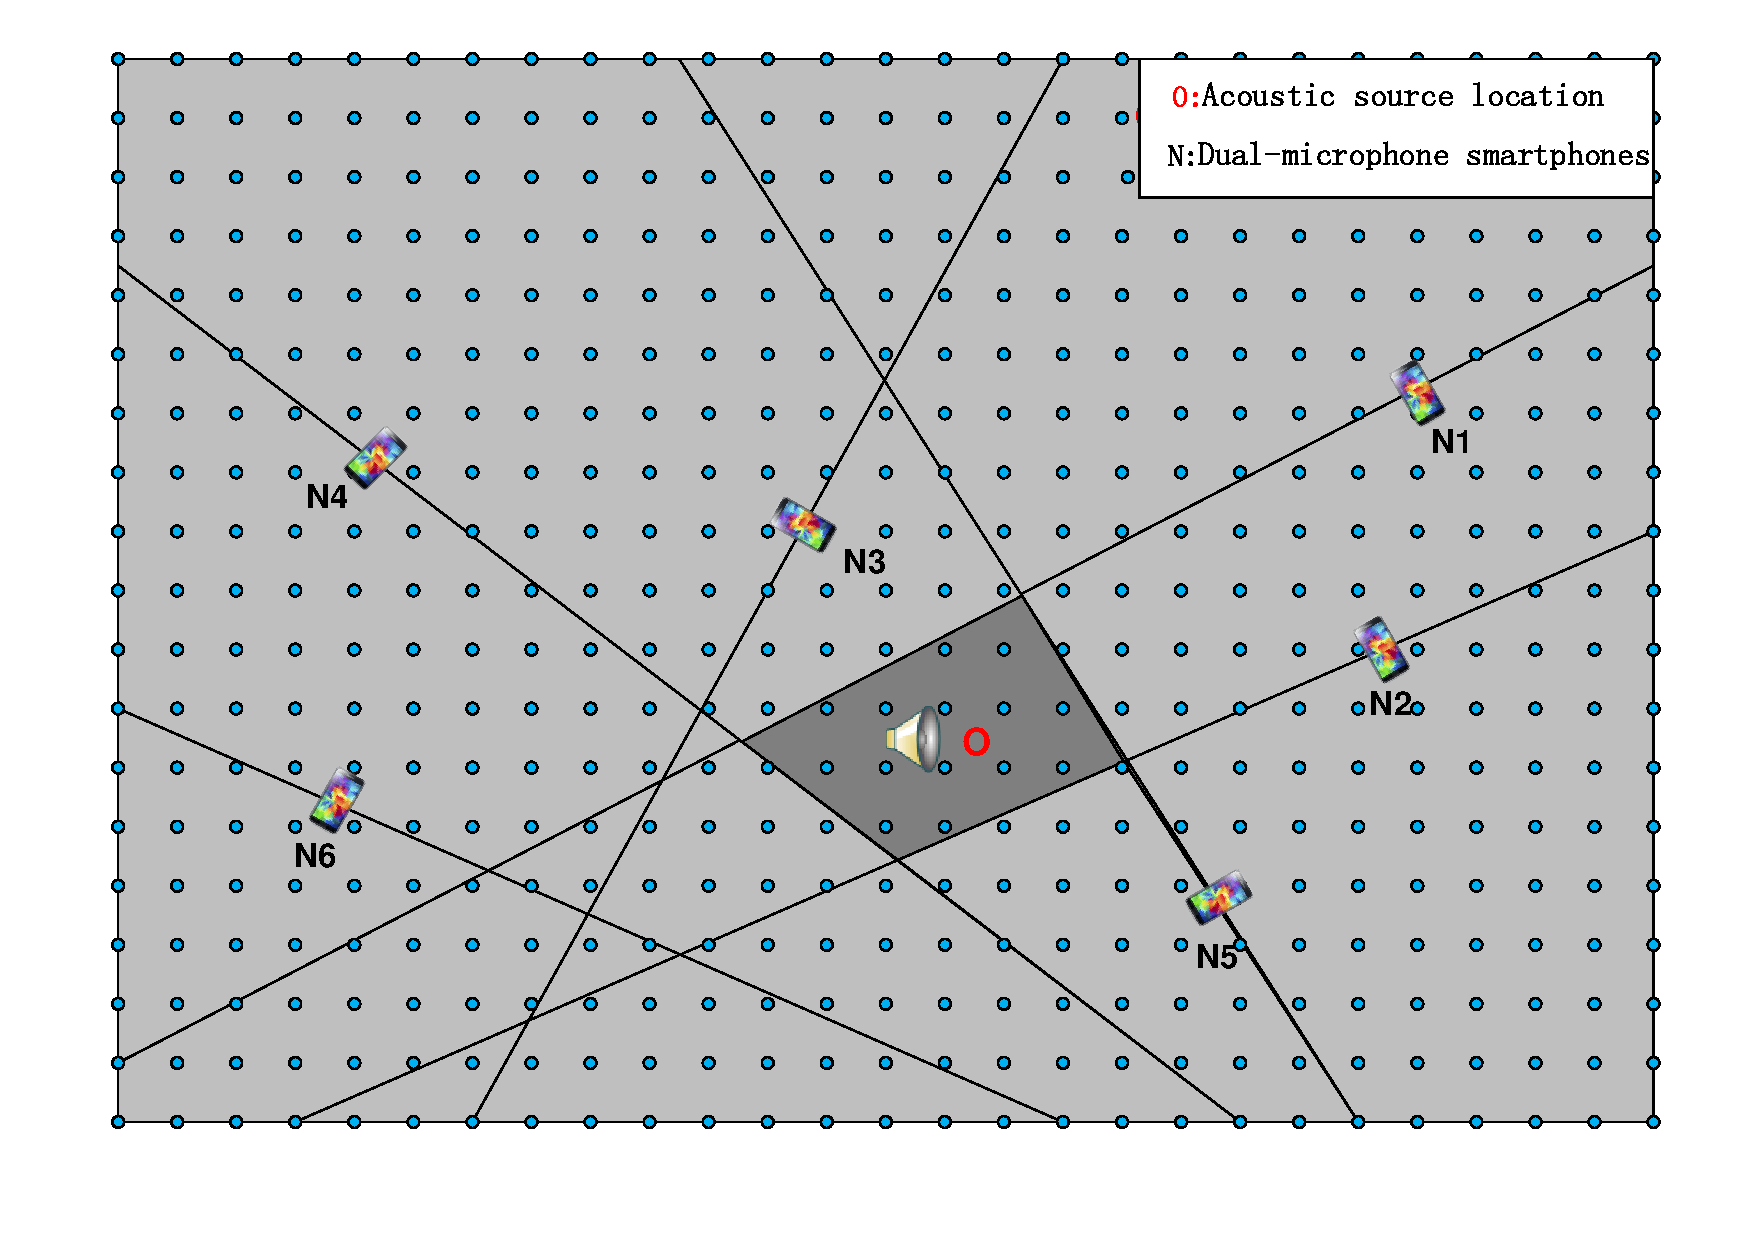
\includegraphics[width=6cm,height=4.0cm]{image/b.pdf} 
	\vspace{3mm}
	\caption{System model}
	\label{fig2}
	\vspace{-5mm}
\end{figure}

As is shown in Fig.1, every lines can divide the space into two parts, when the lines increase to $n$, the space can be divided into $\frac{n^2+n+2}{2}$ parts at best. As long as the number of the smartphones is adequate,  the area of the subdomain is adequately accurate to represent the source location. 
Our target is searching for the points in the target subdomain using the 1-bit measure datas. We make the space gridding with large scale, transform the area into a large number of points.
The points inside the target subdomain are sparse compared with the whole points, satisfy the character of compressive sampling.
%As long as we compress the whole points by 1-bit measure data constantly, finally lead to the points in target subdomain. 
We regard the points in the target subdomain as the final target points, utilizing the average of these points to determine the location of the acoustical source.

Here, we talk about our 1-bit CS framework, considering the scene in the 2D space with $n$ points and $m$ smartphones, $n$ is large that can present the whole localization area, all points are ${S} = \{ {poin{t_1}}, \cdots ,{poin{t_i}}, \cdots ,{poin{t_n}}\}$, where any node ${poin{t_i}}$ has its location coordinate denoted as $[{x_i},{y_i}]$. The acoustic event occurs at ${O_s}{\rm{ = [}}{x_s},{y_s}]$. As for the $m$ smartphones, we utilize the midperpendicular of the two microphones, transform them to $m$ lines, where the ${lin{e_i}}$ is described as ${a_i}x+{b_i}y+{c_i}=0$, stipulate $a_i$ is a positive number all the time.  And the data we measure from every smartphone can be defined as
\begin{equation}\label{eq:eps}
D_{i}=
\left\{\begin{matrix}
1 ~~ $if$~~    {a_i}{x_s}+{b_i}{y_s}+{c_i}\geq0,\\
0 ~~ $if$~~   {a_i}{x_s}+{b_i}{y_s}+{c_i}<0,
\end{matrix}\right.
\end{equation}
where $1\leq i \leq m$, our target is to find few points among all the $n$ points when substituting it to the $m$ lines that most approaches to the $D$. Here, we confirm the average of the points to be the real source acoustic location.

We describe the localization model in the matrix form. Coefficient matrix $A$ is denoted as
\begin{equation}\label{eq:eps}
A=\begin{bmatrix}
&a_1  &b_1 &c_1 \\
&a_2  &b_2 &c_2\\
&.&.&. \\
&.&.&. \\
&.&.&. \\
&a_m  &b_m  &c_m
\end{bmatrix}
\end{equation}which indicates the $m$ lines and the point matrix is expressed as
\begin{equation}\label{eq:eps}
S=\begin{bmatrix}
&x_1 &x_2 &. &. &. &x_n \\
&y_2 &y_2 &. &. &. &y_n\\
&1  &1 &. &. &. &1
\end{bmatrix}
\end{equation} 


We represent the unknown target positions on a location grid as a sparse $n\times$1 vector $X$, calculating $X$ to determine whether ${poin{t_i}}$ in the target subdomain, for the points in target area, in matrix $X$ we set their index location as 1, as for other points we give their index value 0. 
To sum up, we conclude our localization model to a formula
\begin{equation}\label{eq:eps}
Sign(ASX)=D
\end{equation}
Provided we solve the matrix $X$, then leading to the points in target subdomain, utilize their average value to represent the location of the acoustic source.  After all concepts are put forward, we introduce the design of our localization method.

